
\chapter{Wyniki działania algorytmu na popularnych zbiorach danych}

\section{Metodologia pomiarów}
	Żeby oszacować trafność klasyfikacji osiąganą przez skonstruowany system konieczne było podzielenie zbioru danych na zbiór uczący i \emph{walidujący}, a w przypadku algorytmu Kernel-GP również wydzielenie ze zbioru uczącego podzbioru \emph{testującego}, używanego do obliczania miary przystosowania (fitness) podczas przebiegu algorytmu genetycznego. Ponieważ sposób podziału zbioru danych ma wpływ na osiąganą trafność klasyfikacji, dokonywano 5 takich podziałów a następnie wyciągano średnią oraz odchylenie standardowe z wyników otrzymanych dla tych podziałów. Ta procedura dotyczyła zarówno testowania algorytmu \emph{Kernel-GP} jak i porównawczych testów klasyfikatora SVM z biblioteki \emph{LibSVM}. Dla obu algorytmów stosowano te same podziały danych, przy czym w przypadku klasyfikatora \emph{LibSVM} ze zbioru uczącego nie wydzielano zbioru testującego.
	
	Algorytm genetyczny jest w swej naturze stochastyczny, korzysta więc z funkcji generujących liczby pseudolosowe. Aby zapewnić powtarzalność wyników i umożliwić ich porównanie ziarno generatora liczb pseudolosowych ustawiono na stałą wartość.

	Aby ocenić skuteczność algorytmu genetycznego w poszukiwaniu optymalnych funkcji jądrowych oraz oszacować optymalną wielkość populacji oraz czas trwania (liczbę ewaluowanych generacji) algorytmu przeprowadzono szereg eksperymentów obliczeniowych, w których uruchamiano algorytm dla coraz to większych wartości tych parametrów. Dla każdego przebiegu algorytmu obliczano i zapisywano kilka miar trafność klasyfikacji zbioru \emph{walidującego}:
	\begin{enumerate}
		\item \definicja{Trafność klasyfikacji} (\english{Accuracy}) - stosunek liczby przypadków ze zbioru walidującego, które zostały zaklasyfikowane poprawnie do liczby wszystkich przepadków w zbiorze walidującym.

		\item \definicja{Miara $ F_{1} $ } (\english{ $ F_{1} $ measure }) - 	miara uwzględniająca zarówno precyzję (\english{precision}) jak i \definicja{kompletność} (\english{recall}) klasyfikacji. Jej wartość jest dana wzorem:
		$$ F_{1} = 2 * \frac{precision * recall}{precision + recall} $$
		Natomiast 
		
		\item \definicja{ \akronim{MCC} \english{Matthews correlation coefficient}} - miara, która bierze pod uwagę wszystkie cztery miary: \english{True Positive} (\akronim{TP}), \english{True Negative}(\akronim{TN}), \english{False Positive} (\akronim{FP}) i \english{False Negative}(\akronim{FN}). Dana wzorem: 
		$$ \text{MCC} = \frac{ TP \times TN - FP \times FN } {\sqrt{ (TP + FP) ( TP + FN ) ( TN + FP ) ( TN + FN ) } } $$
	\end{enumerate}

	Analizując tak zebrane dane można przeanalizować na ile poszukiwanie funkcji jądrowej przez algorytm genetyczny było podobne do losowego przeszukiwania a na ile było ono zbieżne. W pierwszym przypadku na wyniki osiągane przez algorytm powinna mieć wpływ przede wszystkim wielkość populacji, w drugim również liczba generacji przez które poszukiwano rozwiązania. W szczególności ciekawym przypadkiem jest ten, gdy liczba generacji wynosi 1, czyli cały algorytm ogranicza się do wygenerowania populacji losowych osobników i wybrania jednego z nich - w tym przypadku algorytm genetyczny sprowadza się do losowego poszukiwania rozwiązania. Porównując różnicę w trafności osiąganej w trakcie jednej generacji i coraz większej ich liczby można ocenić czy proces ewolucyjny przebiega poprawnie. 
	
\section{Opis zbiorów danych}
	Do oceny pracy algorytmu użyto standardowych zbiorów danych służących do testowania systemów maszynowego uczenia się, dostępnych na stronie biblioteki \emph{LIBSVM} \cite{chang_libsvm:_2011}  oraz w repozytorium UCI  [\ref{url:uci}]. Zbiory zostały opisane w tabelce \ref{tab:datasets}. Użyte nazwy zbiorów są zgodne z tymi ze strony libsvm [\ref{url:libsvm}].

\begin{table}[ht]
	\caption{Zbiory danych użyte do testowania systemu.\label{tab:datasets}} 	
	\begin{tabular}{|p{2cm}|c|p{1.5cm}|p{1.5cm}|p{1.5cm}|p{1.5cm}|p{1.5cm}|}
		\hline 
		Nazwa zbioru & Liczba klas & \hspace{0pt} Liczba atrybutów & \hspace{0pt} Wielkość zbioru & \hspace{0pt} Wielkość zbioru uczącego & \hspace{0pt}Wielkość zbioru testującego & \hspace{0pt} Wielkość zbioru walidującego \\
		\hline 
		Iris & 3 & 4 & 150 & 68 & 33 & 49  \\ 
		\hline 
		Letter & 26 & 16 & 15000 & 9000 & 4400 & 6600\\ 
		\hline 
		DNA & 3 & 180 & 2000 & 1435 & 700 & 1051 \\ 
		\hline 
		Vowel & 11 & 10 & 528 & 447 & 217 & 326 \\ 
		\hline
		Breast cancer & 2 & 10 & 683 & 343 & 170 & 170 \\ 
		\hline
		heart & 2 & 13 & 270 & 136 & 67 & 67 \\ 
		\hline
	\end{tabular} 	
\end{table}

\begin{table}[ht]
\caption{Zbiory danych użyte do testowania systemu.\label{tab:datasets2}} 	
	\begin{tabular}{|p{2.5cm}|p{2.5cm}|p{2.5cm}|p{1.5cm}|p{3cm}|}
	\hline 
	Nazwa zbioru & Liczba atrybutów ciągłych & Liczba atrybutów nominalnych & Liczba klas & Proporcje klas \\ 
	\hline 
	Breast Cancer & 10 & 0 & 2 & 239/444 \\ 
	\hline 
	Heart  & 7 & 6 & 2 & 150/120  \\ 
	\hline 
	DNA & 0 & 180 & 3 & 464/485/1051  \\ 
	\hline 
	Vowel & 10 & 0 & 11 & Każda klasa 48 razy \\ 
	\hline 
	\end{tabular} 
\end{table}

	
\FloatBarrier
\section{Trafność klasyfikacji}
	Jak widać na rysunkach \ref{fig:acc-iris}-\ref{fig:acc-letter-detailed} sprawność algorytmu zależy mocno od konkretnego zbioru danych. Na przykład zbiór IRIS jest na tyle łatwy w klasyfikacji, że ciężko jest poprzez dobranie optymalnej funkcji jądrowej polepszyć znacznie wyniki klasyfikacji.
	Na osiąganą trafność klasyfikacji wpływ ma też podział zbioru danych na testujący, uczący i walidujący - widać to po odchyleniu standardowym widocznym na wykresach.
	
	\subsubsection{Monotoniczność funkcji trafności}
	
	Miejscami funkcja trafności nie jest monotoniczna, a ściślej niemalejąca, względem liczby generacji oraz wielkości populacji (co widać np. na wykresach \ref{fig:acc-iris-detailed} i \ref{fig:acc-vowel-detailed}). Wydawałoby się, że tak być nie powinno (algorytm genetyczny zwraca najlepszego osobnika z całego swojego przebiegu, więc wszystkie osobniki, które pojawiły się podczas przebiegu z 5 generacjami pojawią się podczas przebiegu z 7 generacjami, więc trafność dla przebiegu z 7 generacjami powinna być co najmniej tak dobra jak dla przebiegu z 5 generacjami). Jednak może się tak zdarzyć ze względu na to, że trafność pokazana na wykresach to trafność klasyfikacji zbioru walidującego, natomiast trafność użyta przez algorytm genetyczny jako miara dostosowania (\english{fitness}) to trafność klasyfikacji zbioru testującego. Widać to na wykresie \ref{fig:fit-iris-detailed}, który przedstawia wartość przystosowania dla tych samych danych, dla których na wykresie \ref{fig:acc-iris-detailed} jest pokazana trafność klasyfikacji na zbiorze walidującym - tutaj funkcja wykazuje mniej braku monotoniczności. 
	
	Zatem przynajmniej część braku monotoniczności funkcji trafności na zbiorze walidującym wynika z przeuczenia algorytmu - znaleziona przez algorytm genetyczny funkcja jądrowa lepiej sprawdza się przy klasyfikacji zbioru testującego niż walidującego. Nie jest to jednak jedyna przyczyna braku monotoniczności - widać to na wykresie \ref{fig:fit-vowel-detailed} przedstawiającym wartość funkcji przystosowania dla zbioru \emph{vowel} - jej przebieg jest bardzo podobny do przebiegu ukazanej na rys. \ref{fig:acc-vowel-detailed} funkcji trafności klasyfikacji zbioru walidującego na tym samym zbiorze. Co więc jest przyczyną braku monotoniczności? Warto zauważyć, że funkcja jest niemalejąca ze względu na ilość generacji oraz że dla jednej generacji funkcja jest monotoniczna. Sugeruje to, że "winnym" może być selekcja - w praktyce nie zachodzi ono w przypadku gdy algorytm genetyczny działa przez jedną generację.
    
    \begin{figure}
		
\includegraphics[scale=0.50]{figures/functions/func1}
		\caption{Funkcja z pierwszej generacji, która w przebiego z wielkością populacji 4 osiągnęła fitness $0.4242424$. Przodek funkcji z rys.\ref{fig:func2} \label{fig:func1}}
	\end{figure}
	
	\begin{figure}
		
\includegraphics[scale=0.60]{figures/functions/func2}
		\caption{Funkcja z trzeciej generacji, która w przebiego z wielkością populacji 4 osiągnęła fitness $0.78030306$. Potomek funkcji z rys.\ref{fig:func1}, przodek zwycięskiej funkcji (rys.\ref{fig:func5}) z przebiegu z populacją o wielkości 4.\label{fig:func2}}
	\end{figure}
          
   	\begin{figure}
		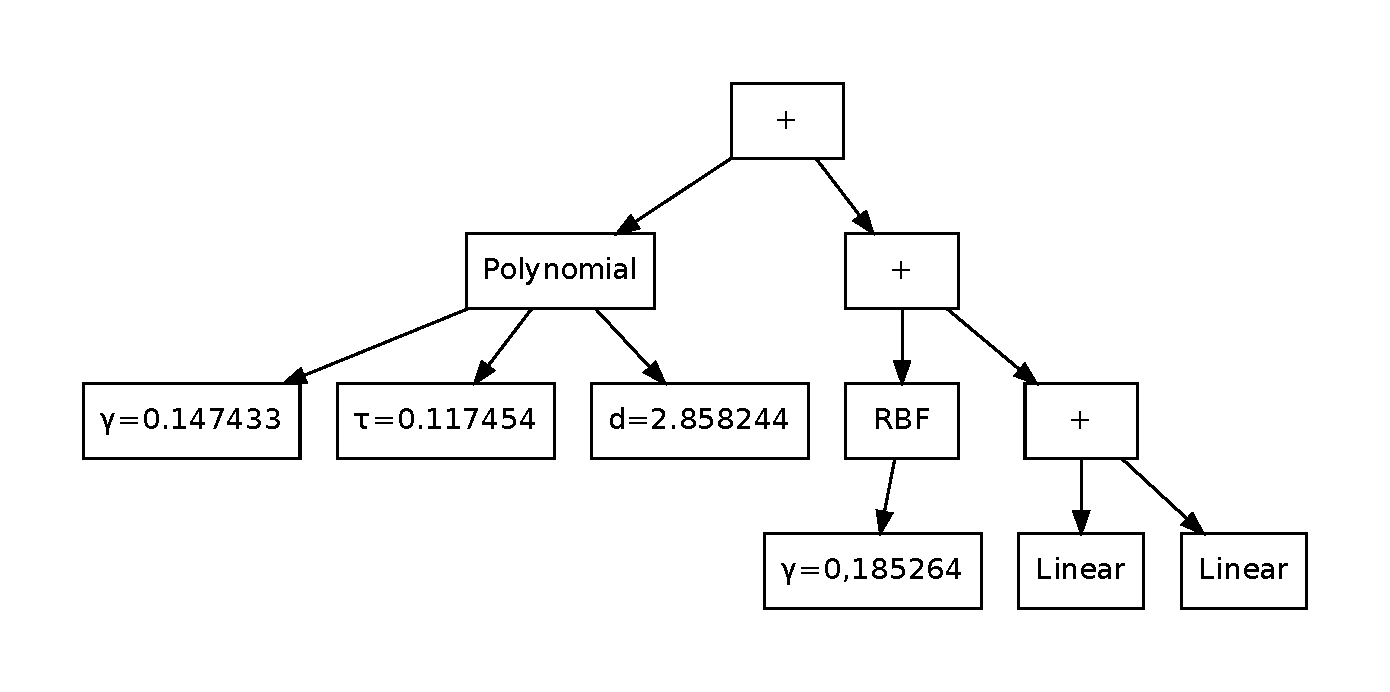
\includegraphics[scale=0.60]{figures/functions/func5}
		\caption{Funkcja z ostatniej generacji w przebiegu z wielkością populacji 4 osiągnęła fitness $0.8333333$. Przodek zwycięskiej funkcji z rys.\ref{fig:func4} \label{fig:func5}}
	\end{figure}          


   	\begin{figure}
		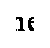
\includegraphics[scale=0.60]{figures/functions/func3}
		\caption{Funkcja z trzeciej generacji, która w przebiegu z wielkością populacji 3 i 4 osiągnęła fitness $0.6515151$. Przodek zwycięskiej funkcji z rys.\ref{fig:func4}\label{fig:func3}}
	\end{figure}                 

    	\begin{figure}
		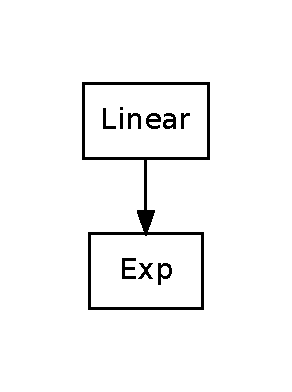
\includegraphics[scale=0.60]{figures/functions/func4}
		\caption{Zwycięska funkcja w przebiegu z populacją wielkości 3, potomek funkcji z rys.\ref{fig:func3}. Osiągnęła fitness $0.9015151$. \label{fig:func4}}
	\end{figure} 	
	
	 Gdy przyjrzeć się dokładnie przebiegowi ewolucji widać, że rzeczywiści tak jest. Dodatkowy osobnik (rys. \ref{fig:func1}), który odróżnia w generacji pierwszej populacje o wielkości 3 i 4 jest przodkiem innego osobnika (rys. \ref{fig:func2}), który w trzeciej generacji osiąga fitness większy niż osobnik (rys. \ref{fig:func3}), który w przypadku populacji wielkości 3 był przodkiem osobnika (rys. \ref{fig:func4}), który to okazał się najlepszym podczas przebiegu całego algorytmu. W rezultacie tego "geny" potencjalnego zwycięzcy nie przetrwały w przebiegu algorytmu z populacją liczącą 4 osobników. Jak widać osobnik najlepszy we wszystkich generacjach nie musi być wcale potomkiem osobników najlepszych w poszczególnych generacjach - czasem połączenie dwóch osobników przeciętnych może dać osobnika bardzo dobrego. 	

	\begin{figure}
		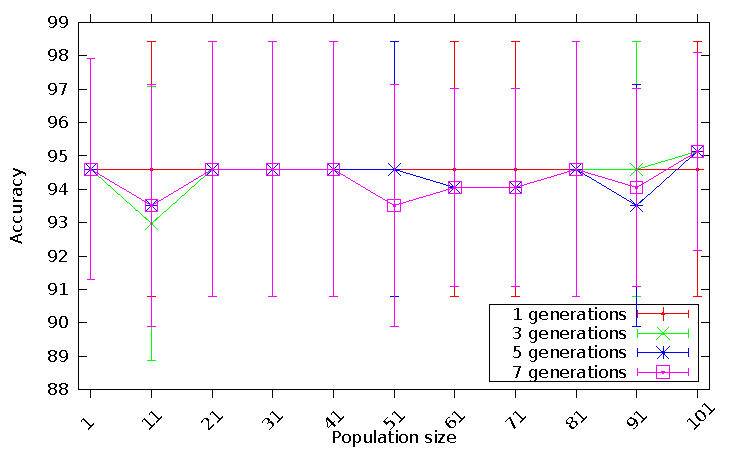
\includegraphics[scale=0.90]{figures/accuracy/accuracy-iris}
		\caption{Dokładność klasyfikacji dla zbioru \emph{iris} w funkcji rozmiaru populacji dla róznych ilości generacji.\label{fig:acc-iris}}
	\end{figure}
	
	\begin{figure}
		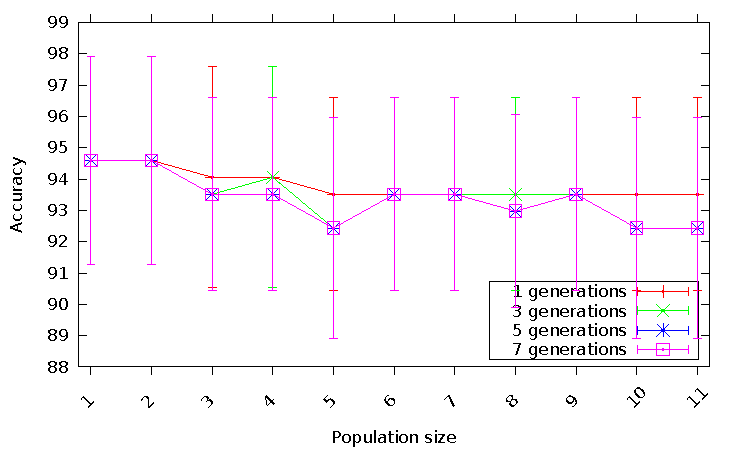
\includegraphics[scale=0.90]{figures/accuracy/accuracy-iris-detailed}
		\caption{Dokładność klasyfikacji dla zbioru \emph{iris} w funkcji rozmiaru populacji dla róznych ilości generacji, dla małych populacji.	\label{fig:acc-iris-detailed}}
	\end{figure}	
	
	
	\begin{figure}
		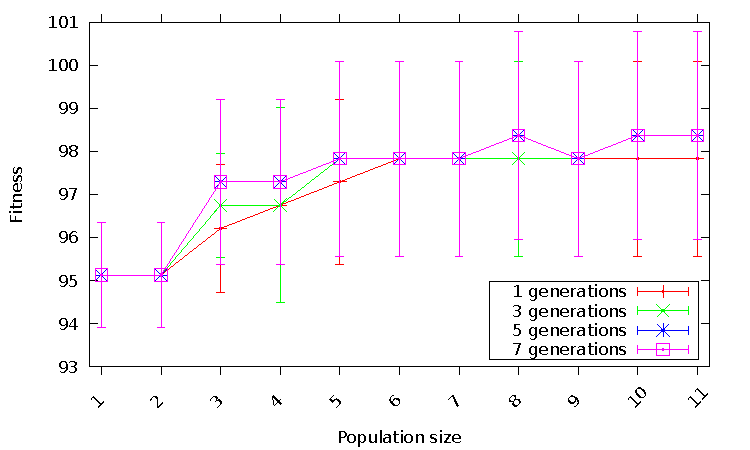
\includegraphics[scale=0.90]{figures/accuracy/fitness-iris-detailed}
		\caption{Najlepsza wartość funkcji przystosowania (\english{fitness})  \emph{iris} w funkcji rozmiaru populacji dla róznych ilości generacji, dla małych populacji.	\label{fig:fit-iris-detailed}}
	\end{figure}	
	
	\begin{figure}
		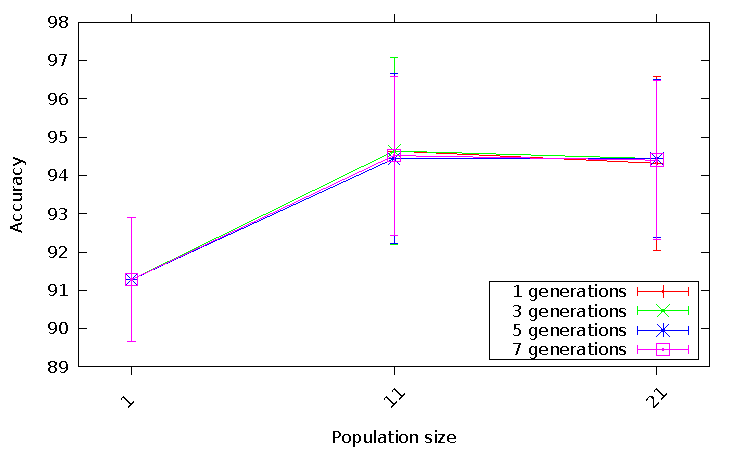
\includegraphics[scale=0.90]{figures/accuracy/accuracy-dna}
		\caption{Dokładność klasyfikacji dla zbioru \emph{DNA} w funkcji rozmiaru populacji dla róznych ilości generacji.\label{fig:acc-dna}}
	\end{figure}
	
	\begin{figure}
		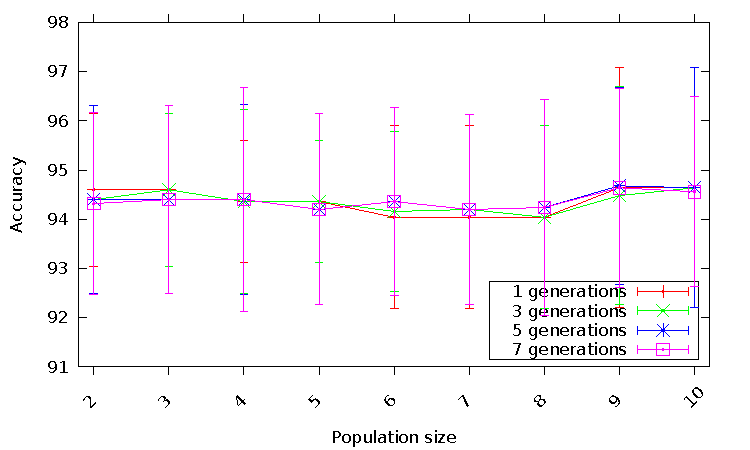
\includegraphics[scale=0.90]{figures/accuracy/accuracy-dna-detailed}
		\caption{Dokładność klasyfikacji dla zbioru \emph{DNA} w funkcji rozmiaru populacji dla róznych ilości generacji, dla małych populacji.\label{fig:acc-dna-detailed}}
	\end{figure}	
	

	\begin{figure}
		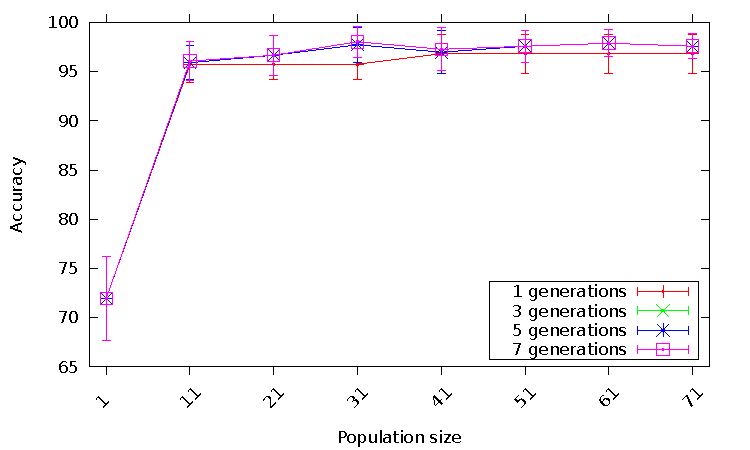
\includegraphics[scale=0.90]{figures/accuracy/accuracy-vowel}
		\caption{Dokładność klasyfikacji dla zbioru \emph{vowel} w funkcji rozmiaru populacji dla róznych ilości generacji.\label{fig:acc-vowel}}
	\end{figure}
		
	\begin{figure}
		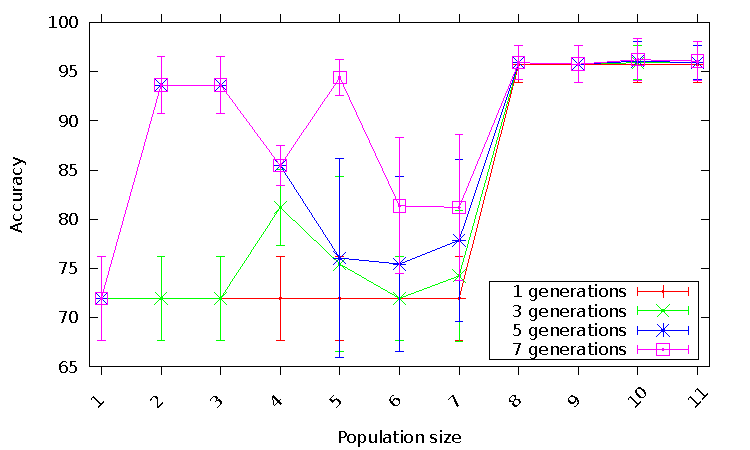
\includegraphics[scale=0.90]{figures/accuracy/accuracy-vowel-detailed}
		\caption{Dokładność klasyfikacji dla zbioru \emph{vowel} w funkcji rozmiaru populacji dla róznych ilości generacji, dla małych populacji.\label{fig:acc-vowel-detailed}}
	\end{figure}
		
	\begin{figure}
		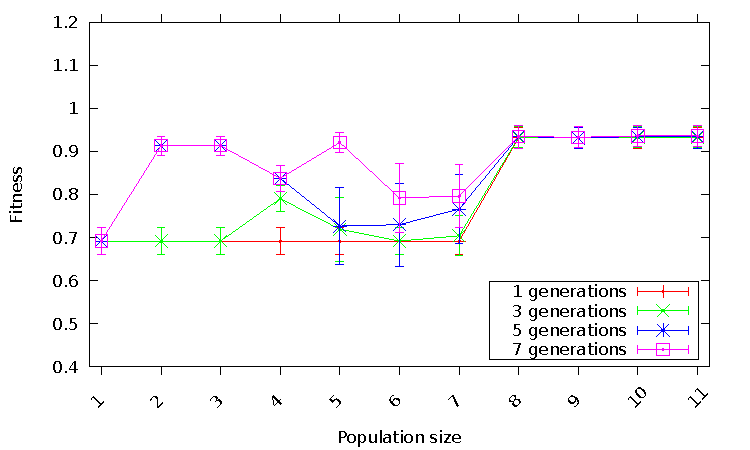
\includegraphics[scale=0.90]{figures/accuracy/fitness-vowel-detailed}
		\caption{Dokładność klasyfikacji dla zbioru \emph{vowel} w funkcji rozmiaru populacji dla róznych ilości generacji, dla małych populacji.\label{fig:fit-vowel-detailed}}
	\end{figure}
	
	
		\begin{figure}
		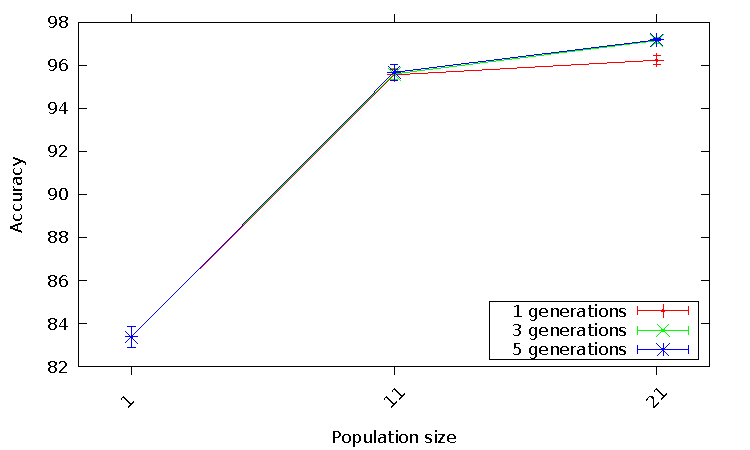
\includegraphics[scale=0.90]{figures/accuracy/accuracy-letter}
		\caption{Dokładność klasyfikacji dla zbioru \emph{letter} w funkcji rozmiaru populacji dla róznych ilości generacji.\label{fig:acc-letter}}
	\end{figure}
	
		
	\begin{figure}
		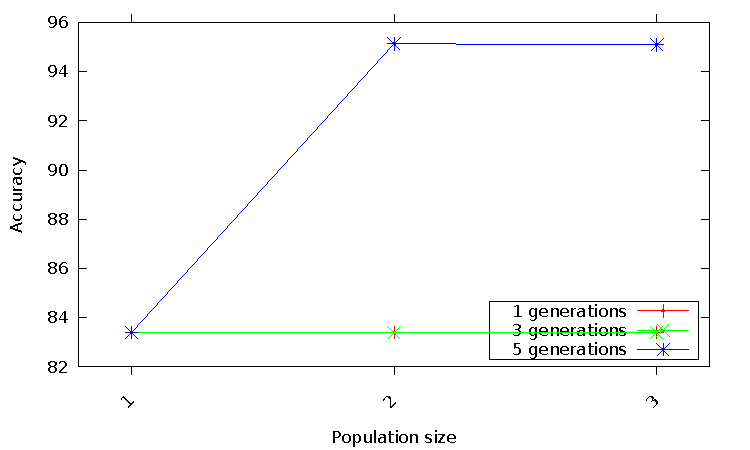
\includegraphics[scale=0.90]{figures/accuracy/accuracy-letter-detailed}
		\caption{Dokładność klasyfikacji dla zbioru \emph{letter} w funkcji rozmiaru populacji dla róznych ilości generacji, dla małych populacji.\label{fig:acc-letter-detailed}}
	\end{figure}
	
	
	\FloatBarrier
		
	\subsection{Porównanie z tradycyjnym algorytmem SVM}
	Na wykresach \ref{fig:acc-iris-svm}-\ref{fig:acc-letter-svm} przedstawiono porównanie trafności klasyfikacji zbioru walidującego przez algorytm SVM z użyciem czterech podstawowych funkcji jądrowych (liniowej, wielomianowej, RBF i sigmoidalnej) i przez stworzony algorytm Kernel-GP.
	W przypadku dwóch zbiorów: \emph{vowel} i \emph{letter} udało się uzyskać polepszenie trafności klasyfikacji względem standardowych funkcji jądrowych. Są to zbiory, dla których standardoy SVM osiąga słabe wyniki - ok. $ 70\% - 80\% $. 

	W przypadku dwóch pozostałych zbiorów niezależnie od użytej funkcji jądrowej osiągana trafność klasyfikacji jest bardzo wysoka - ok. $ 95\% $ - sugeruje to, że zbiory te są dość łatwo separowalne z wyjątkiem $ 5\% $ przypadków.
	
	\begin{figure}
		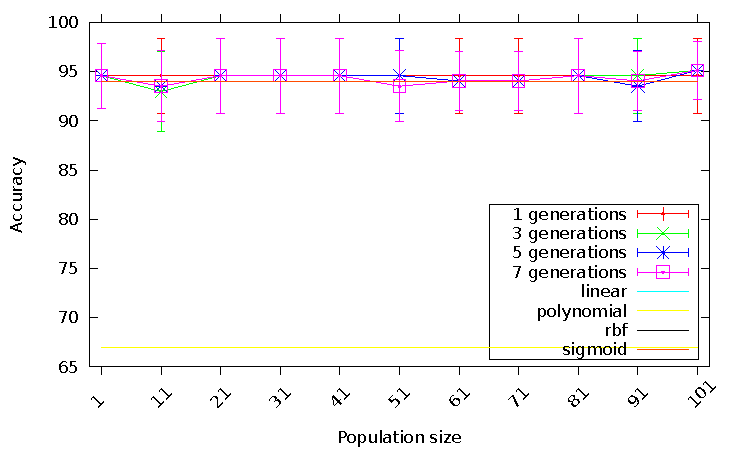
\includegraphics[scale=0.90]{figures/accuracy/accuracy-iris-svm}
		\caption{Porównanie dokładności klasyfikacji dla zbioru \emph{iris} przez algorytm SVM z różnymi funkcjami jądrowymi i algorytm Kernel-GP\label{fig:acc-iris-svm}}
	\end{figure}
	
	\begin{figure}
		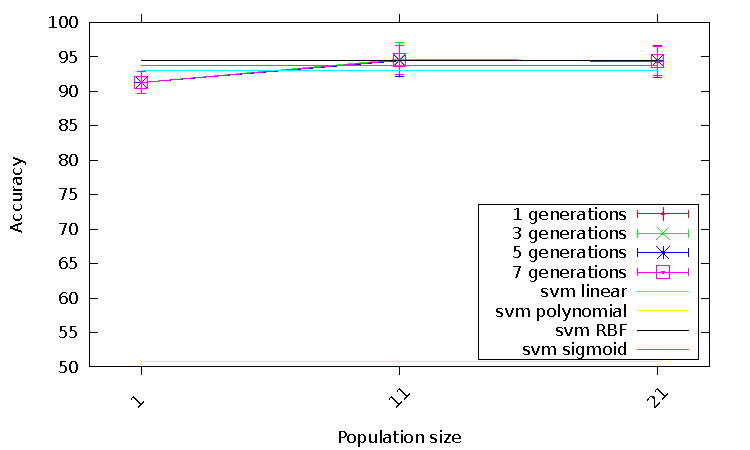
\includegraphics[scale=0.90]{figures/accuracy/accuracy-dna-svm}
		\caption{Porównanie dokładności klasyfikacji dla zbioru \emph{dna} przez algorytm SVM z różnymi funkcjami jądrowymi i algorytm Kernel-GP.\label{fig:acc-dna-svm}}
	\end{figure}	
	
	\begin{figure}
		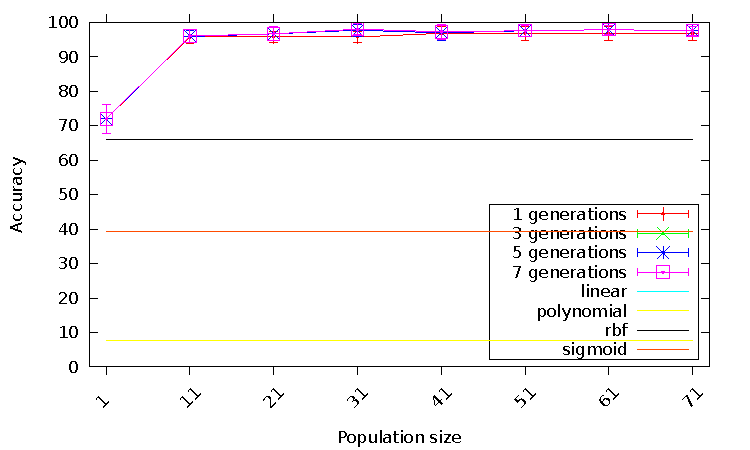
\includegraphics[scale=0.90]{figures/accuracy/accuracy-vowel-svm}
		\caption{Porównanie dokładności klasyfikacji dla zbioru \emph{vowel} przez algorytm SVM z różnymi funkcjami jądrowymi i algorytm Kernel-GP\label{fig:acc-vowel-svm}}
	\end{figure}
	
	\begin{figure}
		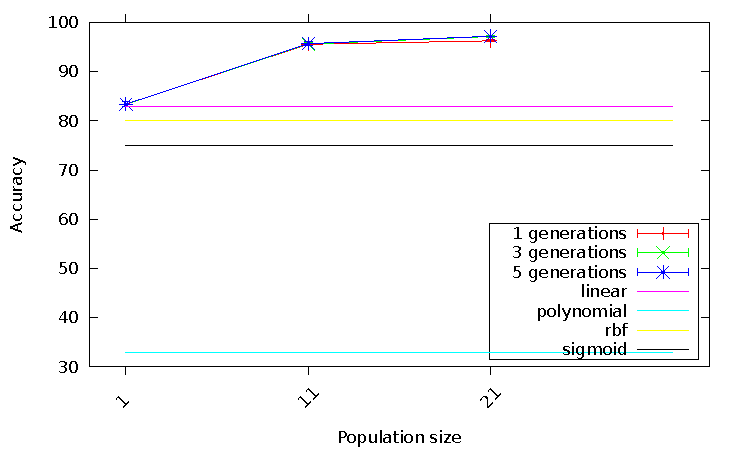
\includegraphics[scale=0.90]{figures/accuracy/accuracy-letter-svm}
		\caption{Porównanie dokładności klasyfikacji dla zbioru \emph{letter} przez algorytm SVM z różnymi funkcjami jądrowymi i algorytm Kernel-GP\label{fig:acc-letter-svm}}
	\end{figure}		
		

\section{Czas wykonania}

\section{Użycie pamięci}

\section{Posdumowanie wyników}

\clearpage
